\documentclass{beamer}

\beamertemplatenavigationsymbolsempty

\mode<presentation>
{
  \usetheme{default}
}

\usepackage[english]{babel}
\usepackage[latin1]{inputenc}
\usepackage{bussproofs}
\usepackage[retainorgcmds]{IEEEtrantools}

% needs debian package texlive-math-extra
\usepackage{stmaryrd} % for \llbracket, \rrbracket

\usepackage{times}
\usepackage[T1]{fontenc}
% Or whatever. Note that the encoding and the font should match. If T1
% does not look nice, try deleting the line with the fontenc.

\usepackage{tikz}
\usetikzlibrary{positioning}
\usetikzlibrary{calc}
\usetikzlibrary{matrix}
\usetikzlibrary{arrows}


\newcommand{\product}{\!\times\!}


\title
{Domains for Algebraic Data Types with Computation Steps}

\author
{Markus~Klinik}

\institute[Radboud University Nijmegen]
{
  Radboud University Nijmegen
}

\date
{August 2014}


\newcommand{\arr}{\rightarrow}
\newcommand{\Arr}{\Rightarrow}
\newcommand{\semantics}[1]{\llbracket #1 \rrbracket}
\newcommand{\semanticsFd}[1]{\semantics{#1}_{F\delta}}
\newcommand{\oftype}[2]{#1\!:\!#2}

\begin{document}

\begin{frame}
  \titlepage
\end{frame}

\begin{frame}{Fixpoints, Sums, Products: Pick Two}

\begin{itemize}
\item What? CCC + Fixpoints + Sums = $\lightning$
\item Who? Huwig and Poign\'e, 1990
\item Why? Raising awareness
\item How? Let's see ...
\end{itemize}

\end{frame}


\begin{frame}[fragile]{Preliminaries}

\begin{definition}
A category is \emph{trivial} iff it has one object with one arrow.
\end{definition}

\begin{definition}
A category has the \emph{fixpoint property} iff every endomorphism has a fixpoint:
$f(Yf) = Yf$
\end{definition}

\begin{center}
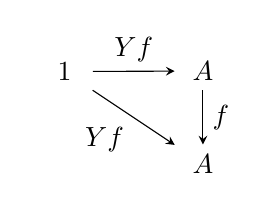
\begin{tikzpicture}
\matrix (m) [matrix of math nodes,row sep=2em,column sep=3em,minimum width=2em]
  {
     1 & A \\
     {} & A \\
  };
  \path[-stealth] (m-1-1) edge node [above] {$Yf$} (m-1-2);
  \path[-stealth] (m-1-1) edge node [below left] {$Yf$} (m-2-2);
  \path[-stealth] (m-1-2) edge node [right] {$f$} (m-2-2);
\end{tikzpicture}
\end{center}

\end{frame}



\begin{frame}[fragile]{Warming Up}

\begin{lemma}
In a category with fixpoints, $0 \cong 1$.
\end{lemma}

\vfill

\begin{center}
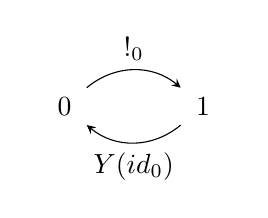
\begin{tikzpicture}
\matrix (m) [matrix of math nodes,row sep=2em,column sep=3em,minimum width=2em]
  {
     0 & 1 \\
  };
  \path[-stealth] (m-1-1) [out=40,in=140] edge node [above] {$!_0$} (m-1-2);
  \path[-stealth] (m-1-2) [out=220, in=320] edge node [below] {$Y(id_0)$} (m-1-1);
\end{tikzpicture}
\end{center}

\end{frame}



\begin{frame}[fragile]{Warming Up}

\begin{lemma}
In a CCC with initial object, for all $A$, $0 \cong 0 \product A$.
\end{lemma}

Existence:
\begin{center}
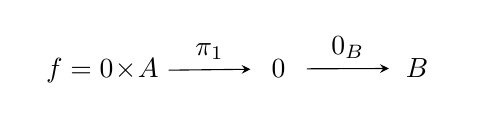
\begin{tikzpicture}
\matrix (m) [matrix of math nodes,row sep=4em,column sep=3em,minimum width=2em]
  {
     f = 0 \product A & 0 & B \\
  };
  \path[-stealth] (m-1-1) edge node [above] {$\pi_1$} (m-1-2);
  \path[-stealth] (m-1-2) edge node [above] {$0_B$} (m-1-3);
\end{tikzpicture}
\end{center}

Uniqueness:
\begin{center}
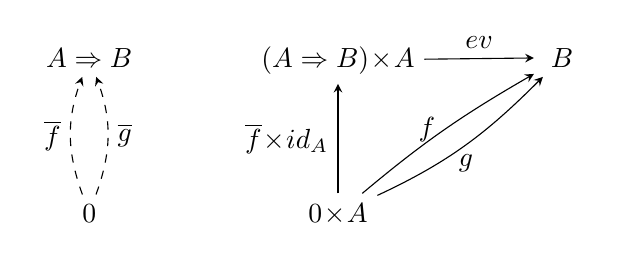
\begin{tikzpicture}
\matrix (m) [matrix of math nodes,row sep=4em,column sep=4em,minimum width=2em]
  {
     A \Arr B & (A \Arr B) \product A & B \\
     0 & 0 \product A \\
  };
  \path[-stealth, dashed] (m-2-1) [out=110,in=250] edge node [left] {$\overline{f}$} (m-1-1);
  \onslide<2->{\path[-stealth, dashed] (m-2-1) [out=70,in=290] edge node [right] {$\overline{g}$} (m-1-1);}
  \path[-stealth] (m-1-2) edge node [above] {$\text{ev}$} (m-1-3)
    (m-2-2) edge node [left] {$\overline{f} \product \text{id}_A$} (m-1-2)
    (m-2-2) [out=40,in=210] edge node [left] {$f$} (m-1-3);
  \onslide<2->{\path[-stealth] (m-2-2) [out=25,in=225] edge node [below] {$g$} (m-1-3);}
\end{tikzpicture}
\end{center}

\end{frame}


\begin{frame}[fragile]{Warming Up}

\begin{theorem}
Any CCC with fixpoints and initial object is trivial.
\end{theorem}

\begin{equation*}
1\ \cong\ 0\ \cong\ 0 \product A\ \cong\ 1 \product A\ \cong\ A
\end{equation*}

\end{frame}


\end{document}
